%%%%%%%%%%%%%%%%%%%%%%%%%%%%%% -*- Mode: Latex -*- %%%%%%%%%%%%%%%%%%%%%%%%%%%%
%% 00slides.tex 
%% Author          : Yaakov Oshman
%% Created On      : Thu Apr 15 22:28:37 2004
%% Last Modified By: Yaakov Oshman
%% Last Modified On: Thu Feb 11 16:39:30 2010
%% Update Count    : 412
%% Status          : Unknown, Use with caution!
%%%%%%%%%%%%%%%%%%%%%%%%%%%%%%%%%%%%%%%%%%%%%%%%%%%%%%%%%%%%%%%%%%%%%%%%%%%%%%%
        
%% PROCESSING THE LATEX FILE (use both input and output file names!):
%%    1. latex file.tex
%%    2. dvips -ta4 -Ppdf file.dvi -o file.ps  (a4 page size)
%%    3. ps2pdf -r1200 file.ps file.pdf (1200 resolution)

       
\documentclass[mathserif]{beamer}
%%\documentclass[gray,handout,mathserif]{beamer}

%%\documentclass[mathserif,allowframebreaks,shrink]{beamer}
%% frame options:
%%  
%% [squeeze] for squeezing vertical space
%% [shrink] for shrinking the content to fit in a single slide
%% \frame[plain]{\frametitle{}...} for plane frame style
%% [allowframebreaks] automatic splitting of frame if content does not
%% fit in a single slide


%\usetheme{split}    % takes more vertical space!!
%\usetheme{Berkeley} % vertical side navigation bar
%\usetheme{Malmoe}
%\usetheme{shadow}
%\usetheme{PaloAlto}  %  side nav bar
%\usetheme{Copenhagen}  %  top nav bar
%\usetheme{Madrid}  %  no nav bar
\usetheme{Boadilla}  % nice and clean, no nav bar, max space!
%\usetheme{montpellier}  %  top tree
%\usetheme{Singapore}  %  top (sort of tree)
%\usetheme{pittsburgh}   % no nav bar, clean, takes more space than Boadilla...
%\usetheme{szeged}

\setbeamertemplate{navigation symbols}{}  %no nav symbols at bottom of PDF
%% or
%% \usenavigationsymbolstemplate{}
%%



\usepackage{eulervm}
%%\usepackage[small]{eulervm}

%%\beamertemplateballitem    %% fancy bulletts

\usepackage{colordvi}  %% texmf/tex/generic/dvips/colordvi.tex (names
                       %% of all predefined colors)

\usepackage{amsmath}
\usepackage{amssymb}
\usepackage{amsfonts}
\usepackage{amsthm}
\usepackage{bm}
\usepackage{xspace}
\usepackage{latexsym}
\usepackage{mathrsfs}
\usepackage{wasysym}
%\usepackage{arydshln}
\usepackage{eulervm}
\usepackage[T1]{fontenc}
\usepackage{aurical}


\graphicspath{{Figures/}}
\DeclareGraphicsRule{*}{eps}{*}{}
%\DeclareGraphicsExtensions{.eps}

\newcommand{\epspath}{}
%\newcommand{\epspath}{g:/usr1/etc/logos/}
   
\newenvironment{slidelist}{\begin{list}{$\bullet$}%
    {\itemsep -0.5ex \topsep -2ex \partopsep 0ex}}{\end{list}}

\newenvironment{smilebullet}{\begin{list}{{\large \green \smiley}}%
{\itemsep 1ex \partopsep 0ex}}{\end{list}}

\newenvironment{frownbullet}{\begin{list}{{\large \green \frownie}}%
{\itemsep 1ex  \partopsep 0ex}}{\end{list}}

\newcommand{\subheading}[1]{\textbf{\textsf{{\textcolor{blue}{#1}}}}}
\newcommand{\subsubheading}[1]{\textbf{\textsf{\textcolor{red}{#1}}}}


\title[BLOM]{{\bf BLOM}: {\bf B}erkeley {\bf L}ibrary for \\ 
  {\bf O}ptimization {\bf M}odeling}
%
\author[S. Vichik, A. Kelman]{Sergey Vichik
%
  ~and~Anthony Kelman }


\date[March 2012]{March, 2012}

\institute[UC Berkeley]{UC Berkeley\\
  Department of Mechanical Engineering\\
  Berkeley, CA \\[1ex]
  sergv@berkeley.edu, \hspace{1em}
}

%

\renewcommand{\include}{\input}       


         
\begin{document}

%
\begin{frame}
  \titlepage
\end{frame}
%

%\begin{frame} \frametitle{Outline}
%  \tableofcontents
%\end{frame}
%
%\include{abstract}
%%\tableofcontents[current]

\begin{frame}
\frametitle{What is BLOM ?}
\begin{itemize}
\item A language of modeling
dynamical nonlinear systems for optimization problems, especially MPC.
\item Support for the following design phases:
\begin{itemize}
\item Developing the model with an intuitive block diagram.
\item Forward simulation and validation of the model.
\item Automatic export of the optimization problem to a solver. 
\end{itemize}
\item Developed to handle non trivial problems
\begin{itemize}
\item C++ or Matlab code generation.
\item Explicit evaluation of Jacobian and Hessian.
\item Proven with problems of tens of thousands variables.
\end{itemize}
\item Eliminates manual problem coding, eases maintenance and assures that the
  same model used for optimization and for simulation.
\end{itemize}
\end{frame}

\begin{frame}
\frametitle{''Hello World'' example}

\centering 
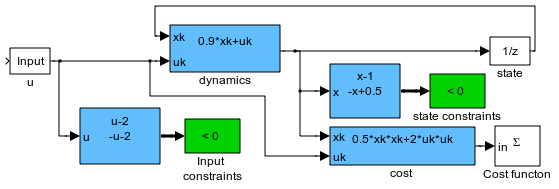
\includegraphics[width = .7\textwidth]{HelloWorld}
\begin {align}
\min_{u_k,x_k}& \sum_k 0.5x_k^2 + 2u_k^2 \notag \\
s.t.:&  -2 \leq u_k \leq 2 \ ; 0.5 \leq x_k \leq 1\ ; x_{k+1}=0.9x_k+u_k \notag
\end{align}


\begin{itemize}
\item The \alert{Functional} block holds expression of the form $\frac{f(x)}{g(x)}$,
   
\item The \alert{Constraint} block marks variable as $\geq 0$ or $\leq 0$.  
\item The continuous or discrete \alert{State} block.
\item The \alert{Cost} block, accumulates cost variables.
\item The \alert{Input/External} variable modifiers marks the control and the
  external variables.
\end{itemize}
\end{frame}

\begin{frame}
\frametitle{The functional block ''Polyblock''}
\begin{itemize}
\item Each polyblock is a polynomial-like function, that is described by two matrices, $A$ and $C$. $C$ holds the
 term coefficients and $A$ defines the functions of variable to participate in
 the term.
\item  The polynomial-like function has the form: $f(x)=\sum_i \prod_j
v_{i,j}(x_i)$.  $v(x_i) \in \left \{ \alert{x^p} _{ p \in \mathbb R}, \alert{ \exp(x)} ,
\alert{\log(x)} \right \}$.
\item Example:
\begin{equation*}
f(x) = 4 x_1^3 + 0.2 x_1^2 x_2^{0.7} - 0.8 x_1 \exp(x_3) + 0.5 \log( x_2)
\label{eq:example_poly}
\end{equation*}

\begin{equation*}
c = \left[\begin{array}{c} c_1 \\ c_2 \\ c_3 \\ c_4 \end{array}\right] 
= \left[\begin{array}{c} 4 \\ 0.2 \\ -0.8 \\ 0.5 \end{array}\right] 
A = \left[\begin{array}{ccc} 3 & 0 & 0  \\ 2 & 0.7 & 0  \\ 1 & 0 & \inf  \\ 0 & -\inf & 0    \end{array}\right].
\label{eq:example_sparserep}
\end{equation*}
\end{itemize}
\end{frame}


\begin{frame}
\frametitle{BLOM work flow}
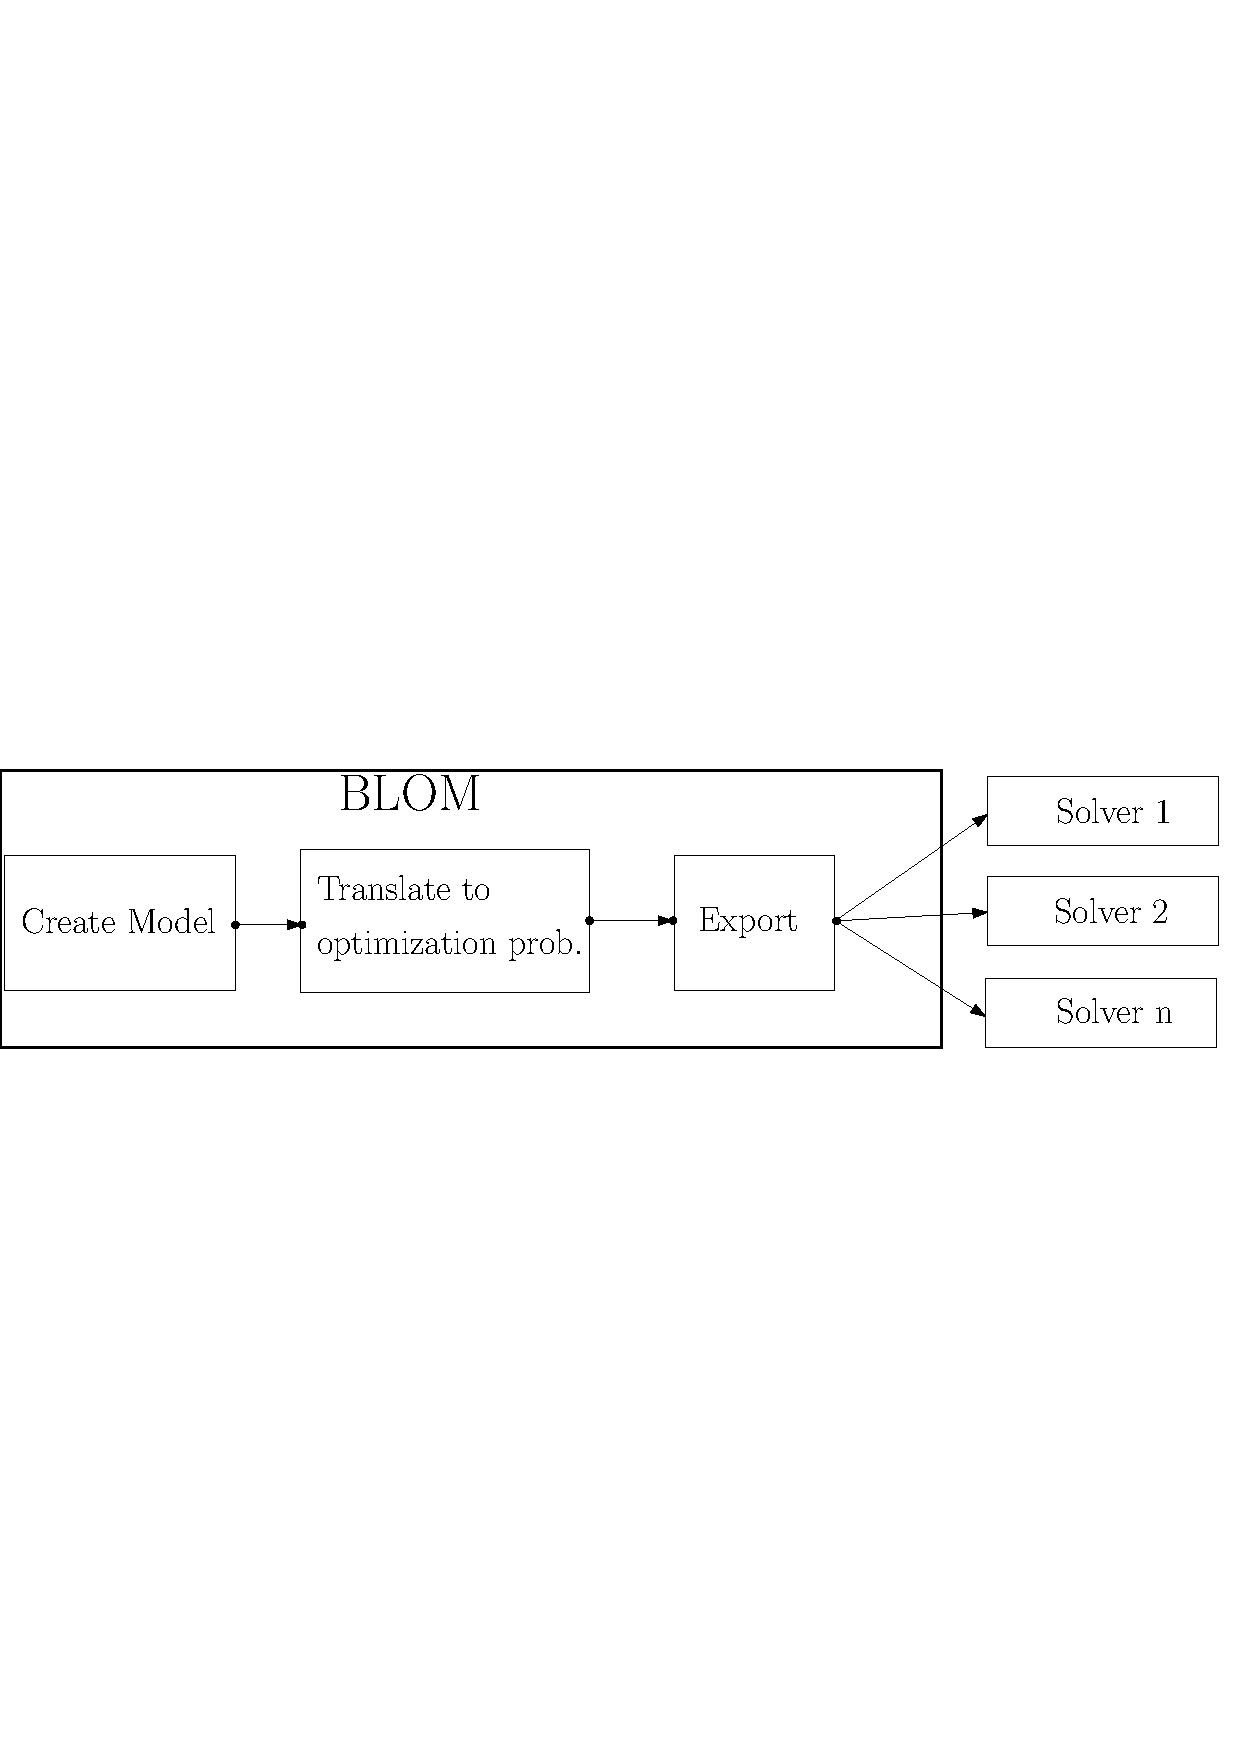
\includegraphics[width=0.9\textwidth]{Flowdgrm}

\begin{itemize}
\item Create model using Simulink with BLOM library. Run and compare the model
  to a reference data. 
\item Translate to optimization problem: {\bf ExtractModel(steps,dt,'RK4');}
\item Export the problem to a solver: e.g. {\bf CreateIpoptCPP }
\end{itemize}

\end{frame}

\begin{frame}
\frametitle{BLOM status and features}
\begin{enumerate}
\item Discrete and continuous models.
\item For continuous model, supports Euler, trapezoidal and RK4 discretization
  (easily expandable).
\item Full vector support.
\item Model developing features: 
\begin{itemize}
\item Color coded constraint violations.
\item Polyblocks display the user defined function.
\item User defined port labeling. 
\end{itemize}
\item Export to IPOPT and fmincon solvers (more to come).
\item Used in joined project with UTRC for large HVAC MPC problem (dynamical
  model with 430 states, typically $\sim30K$ variables in solver). 
%\item High efficiency: with IPOPT the time of evaluation of callback functions
%  (objective, Jacobian, Hessian) is two order of magnitude smaller than the
%  solver time.
\end{enumerate}
\end{frame}

\begin{frame}
\frametitle{BLOM is fast}
\begin{enumerate}
\item Explicit evaluation of the Jacobian and the Hessian. 
\item Jacobian and Hessian are usually very sparse, and they are evaluated according to the sparsity pattern, therefore, only the non-zero elements are computed.
\item BLOM has an efficient C++ plug-in for IPOPT, that evaluates the cost, constraints and the aforementioned Jacobian and Hessian.
\item When used with IPOPT, the solver is a standalone executable, no additional interfacing overhead is added.   
\item When used with IPOPT, the time of cost, constraints, Jacobian and Hessian evaluation is typically less than 10\% of the total solver time. 
\item The solver time is from  milliseconds for small problems to  minutes for tens of thousands variables sparse problems.
\end{enumerate}
\end{frame}


\end{document}

\endinput

